% **** Szablon pracy magisterskiej, licencjackiej lub inżynierskiej ****

\documentclass[polish,12pt,twoside,a4paper]{report}

% *************** Definicje stylu dokumentu ***************

% *********************************************************************************
% W pliku tym zdefiniowany jest wygl¹d dokumentu.
% Zmiany tutaj nie s¹ konieczne o ile nie zamierzasz zmieniaæ wygl¹du dokumentu.
% *********************************************************************************

% *************** Za³adowanie pakietów ***************
\usepackage[a4paper,twoside,left=2.0cm,right=1.5cm,top=1.5cm,bottom=1.5cm]{geometry}
\usepackage[T1]{fontenc}
%\usepackage[cp1250]{inputenc}
\usepackage[utf8]{inputenc}
\usepackage[polish]{babel}
\usepackage{amsmath}
\usepackage{amsfonts}
\usepackage{graphicx}
\usepackage{graphics}
\usepackage{times}
\usepackage{url}
\usepackage{indentfirst}%wciecia a nowych akapitach
\usepackage{float}
\selectlanguage{polish}

%szerokoœœ wciêæ
\setlength{\parindent}{1.25cm}

%numeracja stron
\usepackage{fancyhdr}
\pagestyle{fancy}
\fancyhf{} % usun biezace ustawienia pagin
\fancyhead[LE,RO]{ }
\fancyhead[LO]{ }
\fancyhead[RE]{ }
\fancyfoot[LE,RO]{\small\thepage}
\fancyfoot[LO]{ }
\fancyfoot[RE]{ }
\renewcommand{\headrulewidth}{0.0pt}
\renewcommand{\footrulewidth}{0.0pt}
\addtolength{\headheight}{0.0pt} % pionowy odstep na kreske
\fancypagestyle{plain}{%
\fancyhead{} % usun p. górne na stronach pozbawionych
% numeracji (plain)
\renewcommand{\headrulewidth}{0.0pt} % pozioma kreska
}

% *************** Definicje niektórych kolorów ***************
\usepackage{color}

\definecolor{greenyellow}   {cmyk}{0.15, 0   , 0.69, 0   }
\definecolor{yellow}        {cmyk}{0   , 0   , 1   , 0   }
\definecolor{goldenrod}     {cmyk}{0   , 0.10, 0.84, 0   }
\definecolor{dandelion}     {cmyk}{0   , 0.29, 0.84, 0   }
\definecolor{apricot}       {cmyk}{0   , 0.32, 0.52, 0   }
\definecolor{peach}         {cmyk}{0   , 0.50, 0.70, 0   }
\definecolor{melon}         {cmyk}{0   , 0.46, 0.50, 0   }
\definecolor{yelloworange}  {cmyk}{0   , 0.42, 1   , 0   }
\definecolor{orange}        {cmyk}{0   , 0.61, 0.87, 0   }
\definecolor{burntorange}   {cmyk}{0   , 0.51, 1   , 0   }
\definecolor{bittersweet}   {cmyk}{0   , 0.75, 1   , 0.24}
\definecolor{redorange}     {cmyk}{0   , 0.77, 0.87, 0   }
\definecolor{mahogany}      {cmyk}{0   , 0.85, 0.87, 0.35}
\definecolor{maroon}        {cmyk}{0   , 0.87, 0.68, 0.32}
\definecolor{brickred}      {cmyk}{0   , 0.89, 0.94, 0.28}
\definecolor{red}           {cmyk}{0   , 1   , 1   , 0   }
\definecolor{orangered}     {cmyk}{0   , 1   , 0.50, 0   }
\definecolor{rubinered}     {cmyk}{0   , 1   , 0.13, 0   }
\definecolor{wildstrawberry}{cmyk}{0   , 0.96, 0.39, 0   }
\definecolor{salmon}        {cmyk}{0   , 0.53, 0.38, 0   }
\definecolor{carnationpink} {cmyk}{0   , 0.63, 0   , 0   }
\definecolor{magenta}       {cmyk}{0   , 1   , 0   , 0   }
\definecolor{violetred}     {cmyk}{0   , 0.81, 0   , 0   }
\definecolor{rhodamine}     {cmyk}{0   , 0.82, 0   , 0   }
\definecolor{mulberry}      {cmyk}{0.34, 0.90, 0   , 0.02}
\definecolor{redviolet}     {cmyk}{0.07, 0.90, 0   , 0.34}
\definecolor{fuchsia}       {cmyk}{0.47, 0.91, 0   , 0.08}
\definecolor{lavender}      {cmyk}{0   , 0.48, 0   , 0   }
\definecolor{thistle}       {cmyk}{0.12, 0.59, 0   , 0   }
\definecolor{orchid}        {cmyk}{0.32, 0.64, 0   , 0   }
\definecolor{darkorchid}    {cmyk}{0.40, 0.80, 0.20, 0   }
\definecolor{purple}        {cmyk}{0.45, 0.86, 0   , 0   }
\definecolor{plum}          {cmyk}{0.50, 1   , 0   , 0   }
\definecolor{violet}        {cmyk}{0.79, 0.88, 0   , 0   }
\definecolor{royalpurple}   {cmyk}{0.75, 0.90, 0   , 0   }
\definecolor{blueviolet}    {cmyk}{0.86, 0.91, 0   , 0.04}
\definecolor{periwinkle}    {cmyk}{0.57, 0.55, 0   , 0   }
\definecolor{cadetblue}     {cmyk}{0.62, 0.57, 0.23, 0   }
\definecolor{cornflowerblue}{cmyk}{0.65, 0.13, 0   , 0   }
\definecolor{midnightblue}  {cmyk}{0.98, 0.13, 0   , 0.43}
\definecolor{navyblue}      {cmyk}{0.94, 0.54, 0   , 0   }
\definecolor{royalblue}     {cmyk}{1   , 0.50, 0   , 0   }
\definecolor{blue}          {cmyk}{1   , 1   , 0   , 0   }
\definecolor{cerulean}      {cmyk}{0.94, 0.11, 0   , 0   }
\definecolor{cyan}          {cmyk}{1   , 0   , 0   , 0   }
\definecolor{processblue}   {cmyk}{0.96, 0   , 0   , 0   }
\definecolor{skyblue}       {cmyk}{0.62, 0   , 0.12, 0   }
\definecolor{turquoise}     {cmyk}{0.85, 0   , 0.20, 0   }
\definecolor{tealblue}      {cmyk}{0.86, 0   , 0.34, 0.02}
\definecolor{aquamarine}    {cmyk}{0.82, 0   , 0.30, 0   }
\definecolor{bluegreen}     {cmyk}{0.85, 0   , 0.33, 0   }
\definecolor{emerald}       {cmyk}{1   , 0   , 0.50, 0   }
\definecolor{junglegreen}   {cmyk}{0.99, 0   , 0.52, 0   }
\definecolor{seagreen}      {cmyk}{0.69, 0   , 0.50, 0   }
\definecolor{green}         {cmyk}{1   , 0   , 1   , 0   }
\definecolor{forestgreen}   {cmyk}{0.91, 0   , 0.88, 0.12}
\definecolor{pinegreen}     {cmyk}{0.92, 0   , 0.59, 0.25}
\definecolor{limegreen}     {cmyk}{0.50, 0   , 1   , 0   }
\definecolor{yellowgreen}   {cmyk}{0.44, 0   , 0.74, 0   }
\definecolor{springgreen}   {cmyk}{0.26, 0   , 0.76, 0   }
\definecolor{olivegreen}    {cmyk}{0.64, 0   , 0.95, 0.40}
\definecolor{rawsienna}     {cmyk}{0   , 0.72, 1   , 0.45}
\definecolor{sepia}         {cmyk}{0   , 0.83, 1   , 0.70}
\definecolor{brown}         {cmyk}{0   , 0.81, 1   , 0.60}
\definecolor{tan}           {cmyk}{0.14, 0.42, 0.56, 0   }
\definecolor{gray}          {cmyk}{0   , 0   , 0   , 0.50}
\definecolor{black}         {cmyk}{0   , 0   , 0   , 1   }
\definecolor{white}         {cmyk}{0   , 0   , 0   , 0   } 

% *************** Koniec definicji stylu dokumentu ***************


%definicja przydatnych poleceń
\newcommand{\wydzial}{KOLEGIUM INFORMATYKI STOSOWANEJ}
\newcommand{\kierunek}{Kierunek: INFORMATYKA}
\newcommand{\autor}{Filip Walat}
\newcommand{\album}{Nr albumu studenta w67204}
\newcommand{\temat}{Aplikacja pozwalająca na szybkie sprawdzenie wersji serwisów na serwerach Linux}
\newcommand{\promotor}{Dr. Zofia Matusiewicz}
\newcommand{\typpracy}{Praca projektowa technologie programistyczne IoT - Python}
\newcommand{\miasto}{Rzeszów}
\newcommand{\rok}{2024}
\newcommand{\specjalnosc}{Technologie IoT – Internetu Rzeczy}

\begin{document}

% *************** Włączenie definicji pierwszych stron ***************
% *************** Strony tytułowe ***************

% ************************************************************
% W tym miejscu znajduje sie definicja wyglądu pierwszych stron:
% strony tytułowej, strony z oświadczeniem o treści pracy
% i strony ze spisem treści
% ************************************************************
% *************** Strona tytułowa ***************
%umieszczenie logo i nazwy uczelni
\noindent
\parbox{65mm}{
\includegraphics[width=13.0cm, height=3.0cm]{photos/logoWSIiZ.PNG}}

\vspace{10mm}
\begin{center}
{\Large{}\textbf{\wydzial}}
\end{center}
\vspace{10mm}
\noindent
\hspace{30mm}{\Large{}\textbf{\kierunek}}\\

\noindent
\hspace{30mm}{\Large{}\textbf{\specjalnosc}}
\vspace{30mm}
\begin{center}
	{\large{}\autor}\\
	{\large{}\album}\\
	\vspace{15pt}
	{\huge{}\textbf{\textit{\temat}}}\\
	\vspace{20pt}
	{\normalsize{}Prowadzący: \promotor}\\
	\vspace{80pt}
	{\LARGE{}\textbf{\typpracy}}\\
	\vspace{150pt}
	{\large{}\textbf{\miasto {} \rok}}
\end{center}

% pusta zawartość stopki - brak numeru strony
\thispagestyle{empty}

% *************** Strona z oświadczeniem o treści pracy ***************
\newpage
%\text{}

%\thispagestyle{empty}
%\newpage


% *************** Spis treści ***************
\tableofcontents
% pusta zawartość stopki - brak numeru strony
\thispagestyle{empty}
\newpage

% *************** Koniec pliku front.tex ***************


% *************** Część główna pracy ***************
\chapter*{Wstęp}

W dzisiejszych czasach zarządzanie wersjami serwisów na serwerach Linux staje się coraz bardziej skomplikowane z powodu rosnącej liczby serwisów i ich zależności. Codzienne wyzwania związane z utrzymaniem aktualności i bezpieczeństwa systemów wymagają innowacyjnych i efektywnych rozwiązań. Nasz projekt, wykorzystujący zaawansowane technologie Python i framework Flask, ma na celu wprowadzenie kompleksowego systemu do sprawdzania wersji serwisów, który zarówno usprawni zarządzanie serwerami, jak i znacząco podniesie komfort pracy administratorów systemów.

Dążymy do rozwiązania problemów związanych z monitorowaniem wersji serwisów przez automatyzację procesów, stosując nowoczesne biblioteki takie jak Paramiko do bezpiecznego połączenia z serwerami oraz interaktywne rozwiązania frontendowe. Nasze podejście ma na celu nie tylko ułatwienie zarządzania wersjami oprogramowania, ale także zapewnienie bezpieczeństwa i stabilności systemów poprzez szybkie i efektywne aktualizowanie informacji o serwisach. W ten sposób przyczyniamy się do poprawy ogólnej jakości zarządzania infrastrukturą IT, łącząc praktyczne umiejętności programistyczne z realnymi wyzwaniami administracji serwerami.

Poprzez ten projekt chcemy zademonstrować, jak nowoczesne technologie mogą być wykorzystane do automatyzacji i optymalizacji procesów zarządzania systemami informatycznymi, co w efekcie przyniesie korzyści zarówno dla administratorów, jak i użytkowników końcowych.
\addcontentsline{toc}{chapter}{Wstęp}
\newpage
\chapter{Opis założeń projektu}
\section{Cele projektu}

Celem naszego projektu jest stworzenie zaawansowanej aplikacji do sprawdzania wersji serwisów działających na serwerach Linux. Dążymy do zaprojektowania i implementacji aplikacji, która umożliwia administratorom szybkie i łatwe sprawdzenie wersji zainstalowanych serwisów. Projekt ten ma kluczowe znaczenie dla naszych studiów informatycznych, koncentrując się na wykorzystaniu praktycznych umiejętności programistycznych do rozwiązania realnych problemów w zarządzaniu serwerami.

\begin{itemize}
\item \textbf{Jaki jest cel projektu?} Stworzenie aplikacji do zarządzania wersjami serwisów na serwerach Linux, który usprawnia monitorowanie i zarządzanie wersjami oprogramowania.
\item \textbf{Jaki jest problem, który będzie rozwiązywany oraz proszę wskazać podstawowe źródło problemu?} Problemem jest brak zautomatyzowanego narzędzia do monitorowania wersji serwisów na wielu serwerach, co prowadzi do trudności w utrzymaniu aktualności oprogramowania.
\item \textbf{Dlaczego ten problem jest ważny oraz jakie są dowody potwierdzające jego istnienie?} Niezaktualizowane oprogramowanie może prowadzić do problemów z bezpieczeństwem i wydajnością. Automatyzacja tego procesu jest niezbędna do utrzymania stabilności i bezpieczeństwa systemów.
\item \textbf{Co jest niezbędne, aby problem został rozwiązany przez zespół i dlaczego?} Niezbędne jest zastosowanie nowoczesnych technologii i metod programowania, aby stworzyć elastyczny i skalowalny system do monitorowania wersji serwisów.
\item \textbf{W jaki sposób problem zostanie rozwiązany?} Poprzez zaprojektowanie i implementację aplikacji w Pythonie, wykorzystującej framework Flask oraz bibliotekę Paramiko do zarządzania serwerami Linux.
\end{itemize}

\section{Wymagania funkcjonalne i niefunkcjonalne}

\noindent \textbf{Definicja:}

Wymagania funkcjonalne określają konkretną funkcjonalność lub zachowanie aplikacji, które musi zostać zaimplementowane. Obejmują one specyficzne zadania lub funkcje, które aplikacja powiniena być w stanie wykonać, takie jak przetwarzanie danych, wykonanie obliczeń, reakcja na określone wejścia użytkownika, i inne wymagane operacje.

Wymagania niefunkcjonalne dotyczą ogólnych jakości aplikcaji, takich jak wydajność, bezpieczeństwo, skalowalność, niezawodność, łatwość użytkowania, i zgodność ze standardami. Te wymagania nie opisują bezpośrednio działań aplikacji, ale określają atrybuty, które muszą być spełnione, aby aplikacja była użyteczna i efektywna w swoim środowisku pracy.

\section{Wymagania Funkcjonalne}

Wymagania funkcjonalne aplikacji obejmują:

\begin{itemize}
\item Sprawdzanie wersji serwisów: Użytkownik za pomocą prostego interfejsu może szybko zweryfikować, jakie wersje serwisów są zainstalowane na serwerze.
\item Aktualizacja informacji o serwerze: Użytkownik może zaktualizować informacje o serwerze, takie jak lista monitorowanych serwisów.
\item Bezpieczne zakończenie pracy z aplikacją przez użytkownika.
\end{itemize}

\section{Wymagania Niefunkcjonalne}

Wymagania niefunkcjonalne projektu są równie istotne, zapewniając:

\begin{itemize}
\item Skalowalność i wydajność: Aplikacja została zaprojektowana z myślą o obsłudze dużej liczby serwerów i użytkowników, zapewniając płynną pracę nawet przy wysokim obciążeniu, co jest kluczowe dla zapewnienia ciągłości działania.
\item Szybki czas odpowiedzi i efektywność działania aplikacji.
\item Utrzymywalność i łatwość modyfikacji: Kod źródłowy aplikacji jest zgodny z najlepszymi praktykami programistycznymi, co ułatwia wprowadzanie zmian, aktualizacji oraz szybką diagnozę i naprawę ewentualnych błędów.
\item Możliwość przeprowadzania testów jednostkowych i integracyjnych.
\end{itemize}

\section{Oczekiwania jakościowe aplikacji dedykowanej}

Teraz nadchodzi część, w której definiujemy oczekiwania jakościowe aplikacji dedykowanej zarządzania wersjami serwisów. Te atrybuty opisują sposoby, w jakie oczekujemy, że aplikacja będzie się zachowywała:

\begin{itemize}
\item \textbf{Użyteczność produktu:} Aplikacja powinna charakteryzować się intuicyjnym i łatwym w użyciu interfejsem, minimalizującym potrzebę szkoleń i umożliwiającym szybki dostęp do wszystkich kluczowych funkcji.
\item \textbf{Dostępność aplikacji:} Aplikacja powiniena być dostępna 24/7/365, z zapewnieniem ciągłości działania nawet w przypadku awarii czy nieprzewidzianych sytuacji.
\item \textbf{Wydajność aplikacji:} Oczekuje się, że czas odpowiedzi aplikcaji na kluczowe operacje (np. sprawdzanie wersji serwisów) nie będzie przekraczał 10 sekund, a funkcje offline będą dostępne przez co najmniej 24h.
\end{itemize}

\clearpage
\newpage
\chapter{Opis struktury projektu}
\section{Komponenty i Organizacja Aplikacji}

Projekt Systemu Sprawdzania Wersji Serwisów na Serwerach Linux składa się z kilku głównych komponentów:

\begin{itemize}
\item \textbf{Backend}: Flask, Python
\item \textbf{Frontend}: HTML, CSS, JavaScript
\item \textbf{Skomunikowanie z serwerami Linux}: Paramiko do obsługi SSH
\item \textbf{Repozytorium kodu i kontrola wersji}: Git, GitHub
\end{itemize}

Główne skrypty i pliki:

\begin{itemize}
\item \texttt{app.py}: Główny plik aplikacji Flask, zarządza routingiem i logiką backendu.
\item \texttt{handler/watcher.py}: Skrypt do monitorowania zmian w folderze hostów.
\item \texttt{templates/}: Katalog zawierający szablony HTML dla Flask.
\item \texttt{frontend/static/}: Katalog zawierający pliki statyczne takie jak CSS i JavaScript.
\item \texttt{handler/results/}: Katalog przechowujący wyniki wersji serwisów dla poszczególnych hostów.
\item \texttt{handler/fetch/hosts/}: Katalog przechowujący pliki JSON z danymi hostów.
\end{itemize}


Struktura projektu jest zaprojektowana w taki sposób, aby maksymalizować ponowne wykorzystanie kodu i ułatwić rozszerzanie systemu o nowe funkcjonalności.

\section{Opis Techniczny Projektu}

Projekt został zrealizowany w języku Python z wykorzystaniem frameworka Flask do obsługi backendu oraz HTML, CSS i JavaScript do frontendowej części aplikacji. Do zarządzania projektem i kodem źródłowym wykorzystano środowisko Visual Studio Code oraz system kontroli wersji Git.

\section{Instalacja i uruchomienie po stronie serwera}

Aby uruchomić aplikację na serwerze, należy wykonać następujące kroki:

\begin{enumerate}
    \item Sklonuj repozytorium z GitHub:
    \begin{verbatim}
    git clone https://github.com/filwalu/VersionChecker.git
    \end{verbatim}
    \item Przejdź na gałąź \texttt{main}:
    \begin{verbatim}
    git checkout main
    \end{verbatim}
    \item Przejdź do katalogu \texttt{app}:
    \begin{verbatim}
    cd app/
    \end{verbatim}
    \item Utwórz wirtualne środowisko:
    \begin{verbatim}
    python3 -m venv .venv
    \end{verbatim}
    \item Aktywuj wirtualne środowisko:
    \begin{verbatim}
    source .venv/bin/activate
    \end{verbatim}
    \item Zainstaluj wymagane pakiety:
    \begin{verbatim}
    pip3 install -r requirements.txt
    \end{verbatim}
    \item Uruchom aplikację:
    \begin{verbatim}
    python3 app.py
    \end{verbatim}
\end{enumerate}

\section{Po stronie użytkownika}

Aby uzyskać dostęp do aplikacji, użytkownik powinien w przeglądarce internetowej wejść na adres:

\begin{verbatim}
127.0.0.1:5001
\end{verbatim}

\noindent W ten sposób użytkownik połączy się z uruchomioną aplikacją.


\subsection{Wymagania systemowe}

Aplikacja jest zaprojektowana z myślą o niskich wymaganiach sprzętowych:

\begin{itemize}
\item Procesor: 1 GHz lub szybszy.
\item Pamięć RAM: 512 MB.
\item Przestrzeń na dysku: 100 MB.
\item System operacyjny: Linux, Windows, MacOS.
\end{itemize}

\subsection{Mechanizm zarządzania danymi}

Projekt wykorzystuje pliki JSON do przechowywania danych o serwisach i wersjach, co pozwala na prostą i efektywną manipulację danymi bez potrzeby korzystania z zewnętrznych systemów DBMS. Struktura plików JSON jest zaprojektowana w taki sposób, aby umożliwić szybkie odczytywanie i zapisywanie stanu serwisów oraz informacji o wersjach, co zapewnia wysoką wydajność działania systemu.

\section{Repozytorium i System Kontroli Wersji}

Projekt wykorzystuje system kontroli wersji Git, co umożliwia skuteczne zarządzanie historią zmian kodu źródłowego. Repozytorium kodu znajduje się na platformie GitHub pod adresem:\ \url{https://github.com/filwalu/VersionChecker} i będzie dostępne publicznie do dnia 30.09.2024. Bezpieczne połączenie z repozytorium zabezpieczono za pomocą pary kluczy SSH. Poniżej przedstawiono opis użytych poleceń Git:

\begin{enumerate}
\item \texttt{git init} - inicjalizacja nowego repozytorium Git.
\item \texttt{git clone [URL]} - klonowanie repozytorium przy użyciu SSH.
\item \texttt{git add -A} - dodawanie zmian do kolejki commitów.
\item \texttt{git status} - sprawdzanie statusu zmian.
\item \texttt{git commit -m "[wiadomość]"} - commitowanie zmian z opisem.
\item \texttt{git push} - wysyłanie zmian do zdalnego repozytorium przez SSH.
\item \texttt{git merge [branch]} - scalanie zmian z wybranej gałęzi do bieżącej gałęzi.
\end{enumerate}

\clearpage
\newpage
\chapter{Harmonogram Realizacji Projektu}

Harmonogram realizacji projektu został zaplanowany z wykorzystaniem diagramu Gantta, który ilustruje kluczowe etapy rozwoju projektu, ich zależności czasowe oraz alokację zasobów. Poniżej przedstawiono diagram Gantta dla projektu aplikacji pozwalającej na szybkie sprawdzenie wersji serwisów na serwerach Linux.

\begin{figure}[H]
\centering
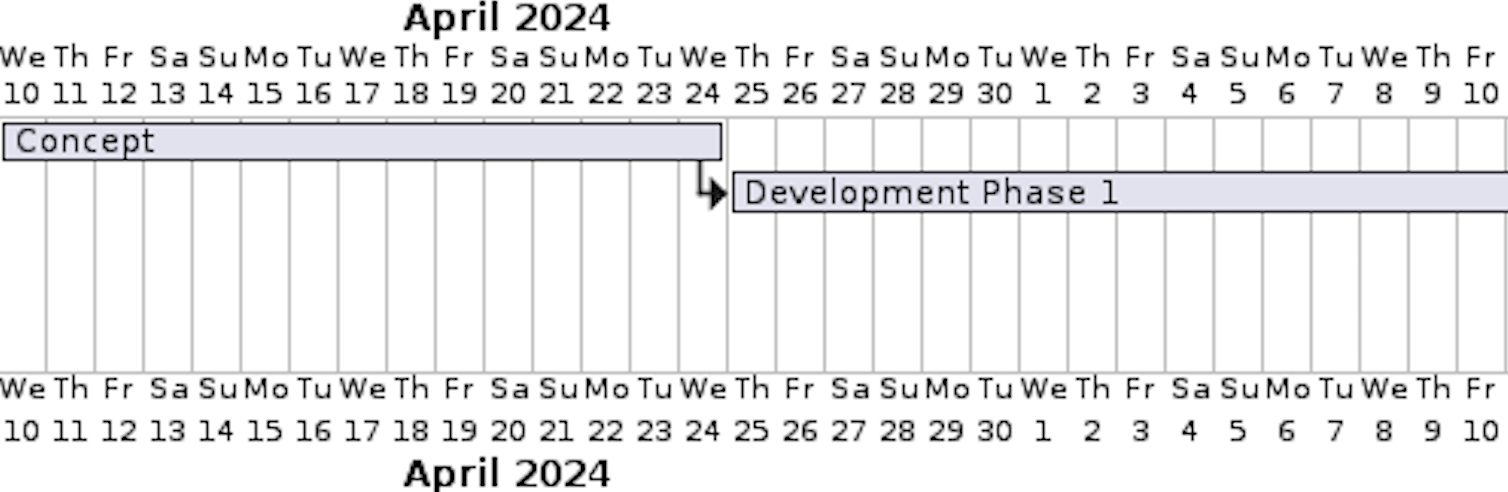
\includegraphics[width=\textwidth]{photos/Gant1.png}
\caption{Diagram Gantta}
\end{figure}
\begin{figure}[H]
\centering
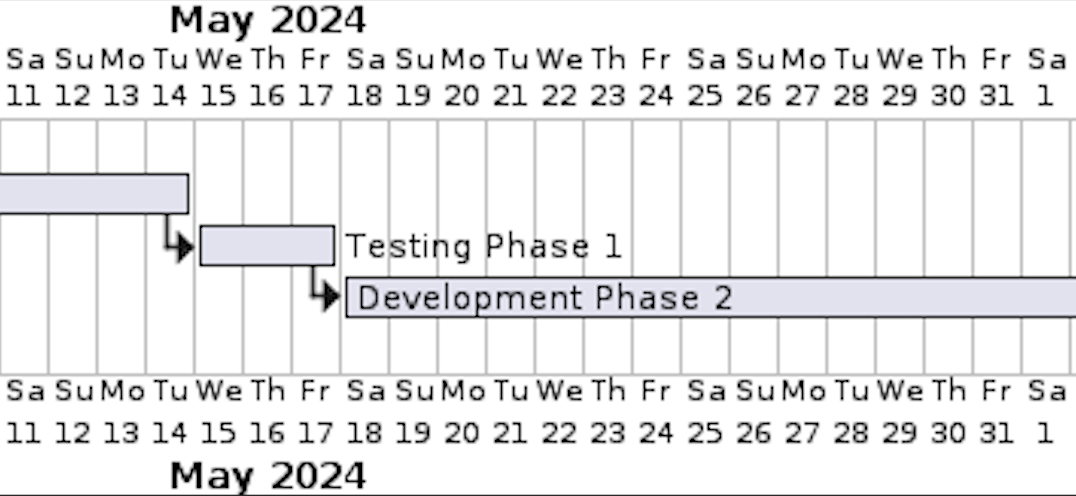
\includegraphics[width=\textwidth]{photos/Gant2.png}
\caption{Diagram Gantta}
\end{figure}
\begin{figure}[H]
\centering
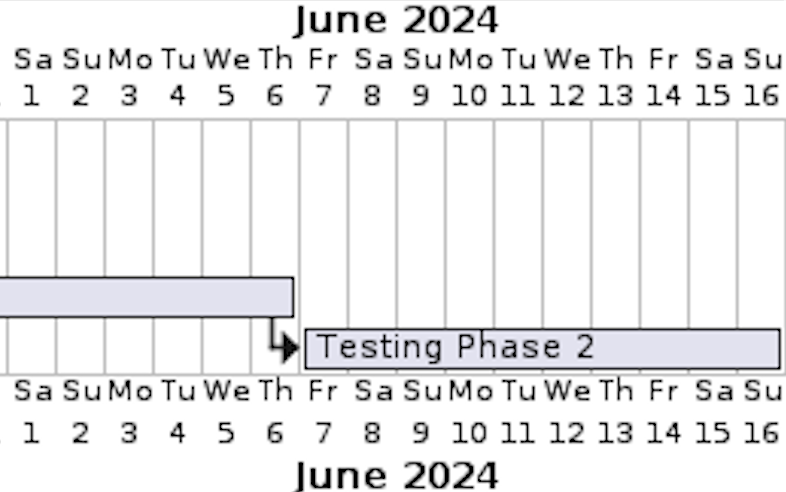
\includegraphics[width=0.80\textwidth]{photos/Gant3.png}
\caption{Diagram Gantta}
\end{figure}

\newpage
\chapter{Prezentacja warstwy użytkowej projektu}

\section{Warstwa Użytkowa Projektu}

Projekt Aplikacji pozwalającej na szybkie sprawdzenie wersji serwisów na serwerach Linux oferuje intuicyjny i prosty w obsłudze interfejs użytkownika, który umożliwia szybkie sprawdzenie wersji serwisów na serwerach Linux.

Aplikacja umożliwia użytkownikom wykonanie następujących akcji:
\begin{itemize}
    \item Sprawdzenie wersji serwisów na danym hoście.
    \item Wywołanie funkcji, która sprawdzi czy wersje serwisów zmieniły się na danym hoście i w razie potrzeby je zaaktualizuje na stronie.
    \item Zmianę wyświetlanych hostów za pomocą przycisków.
\end{itemize}

Interfejs skupia się na minimalizmie i łatwości nawigacji, co pozwala na szybkie odnalezienie potrzebnych informacji i funkcji.

W tej sekcji zostaną umieszczone zrzuty ekranu przedstawiające kluczowe funkcjonalności aplikacji oraz jej interfejs użytkownika.

\begin{figure}[H]
\centering
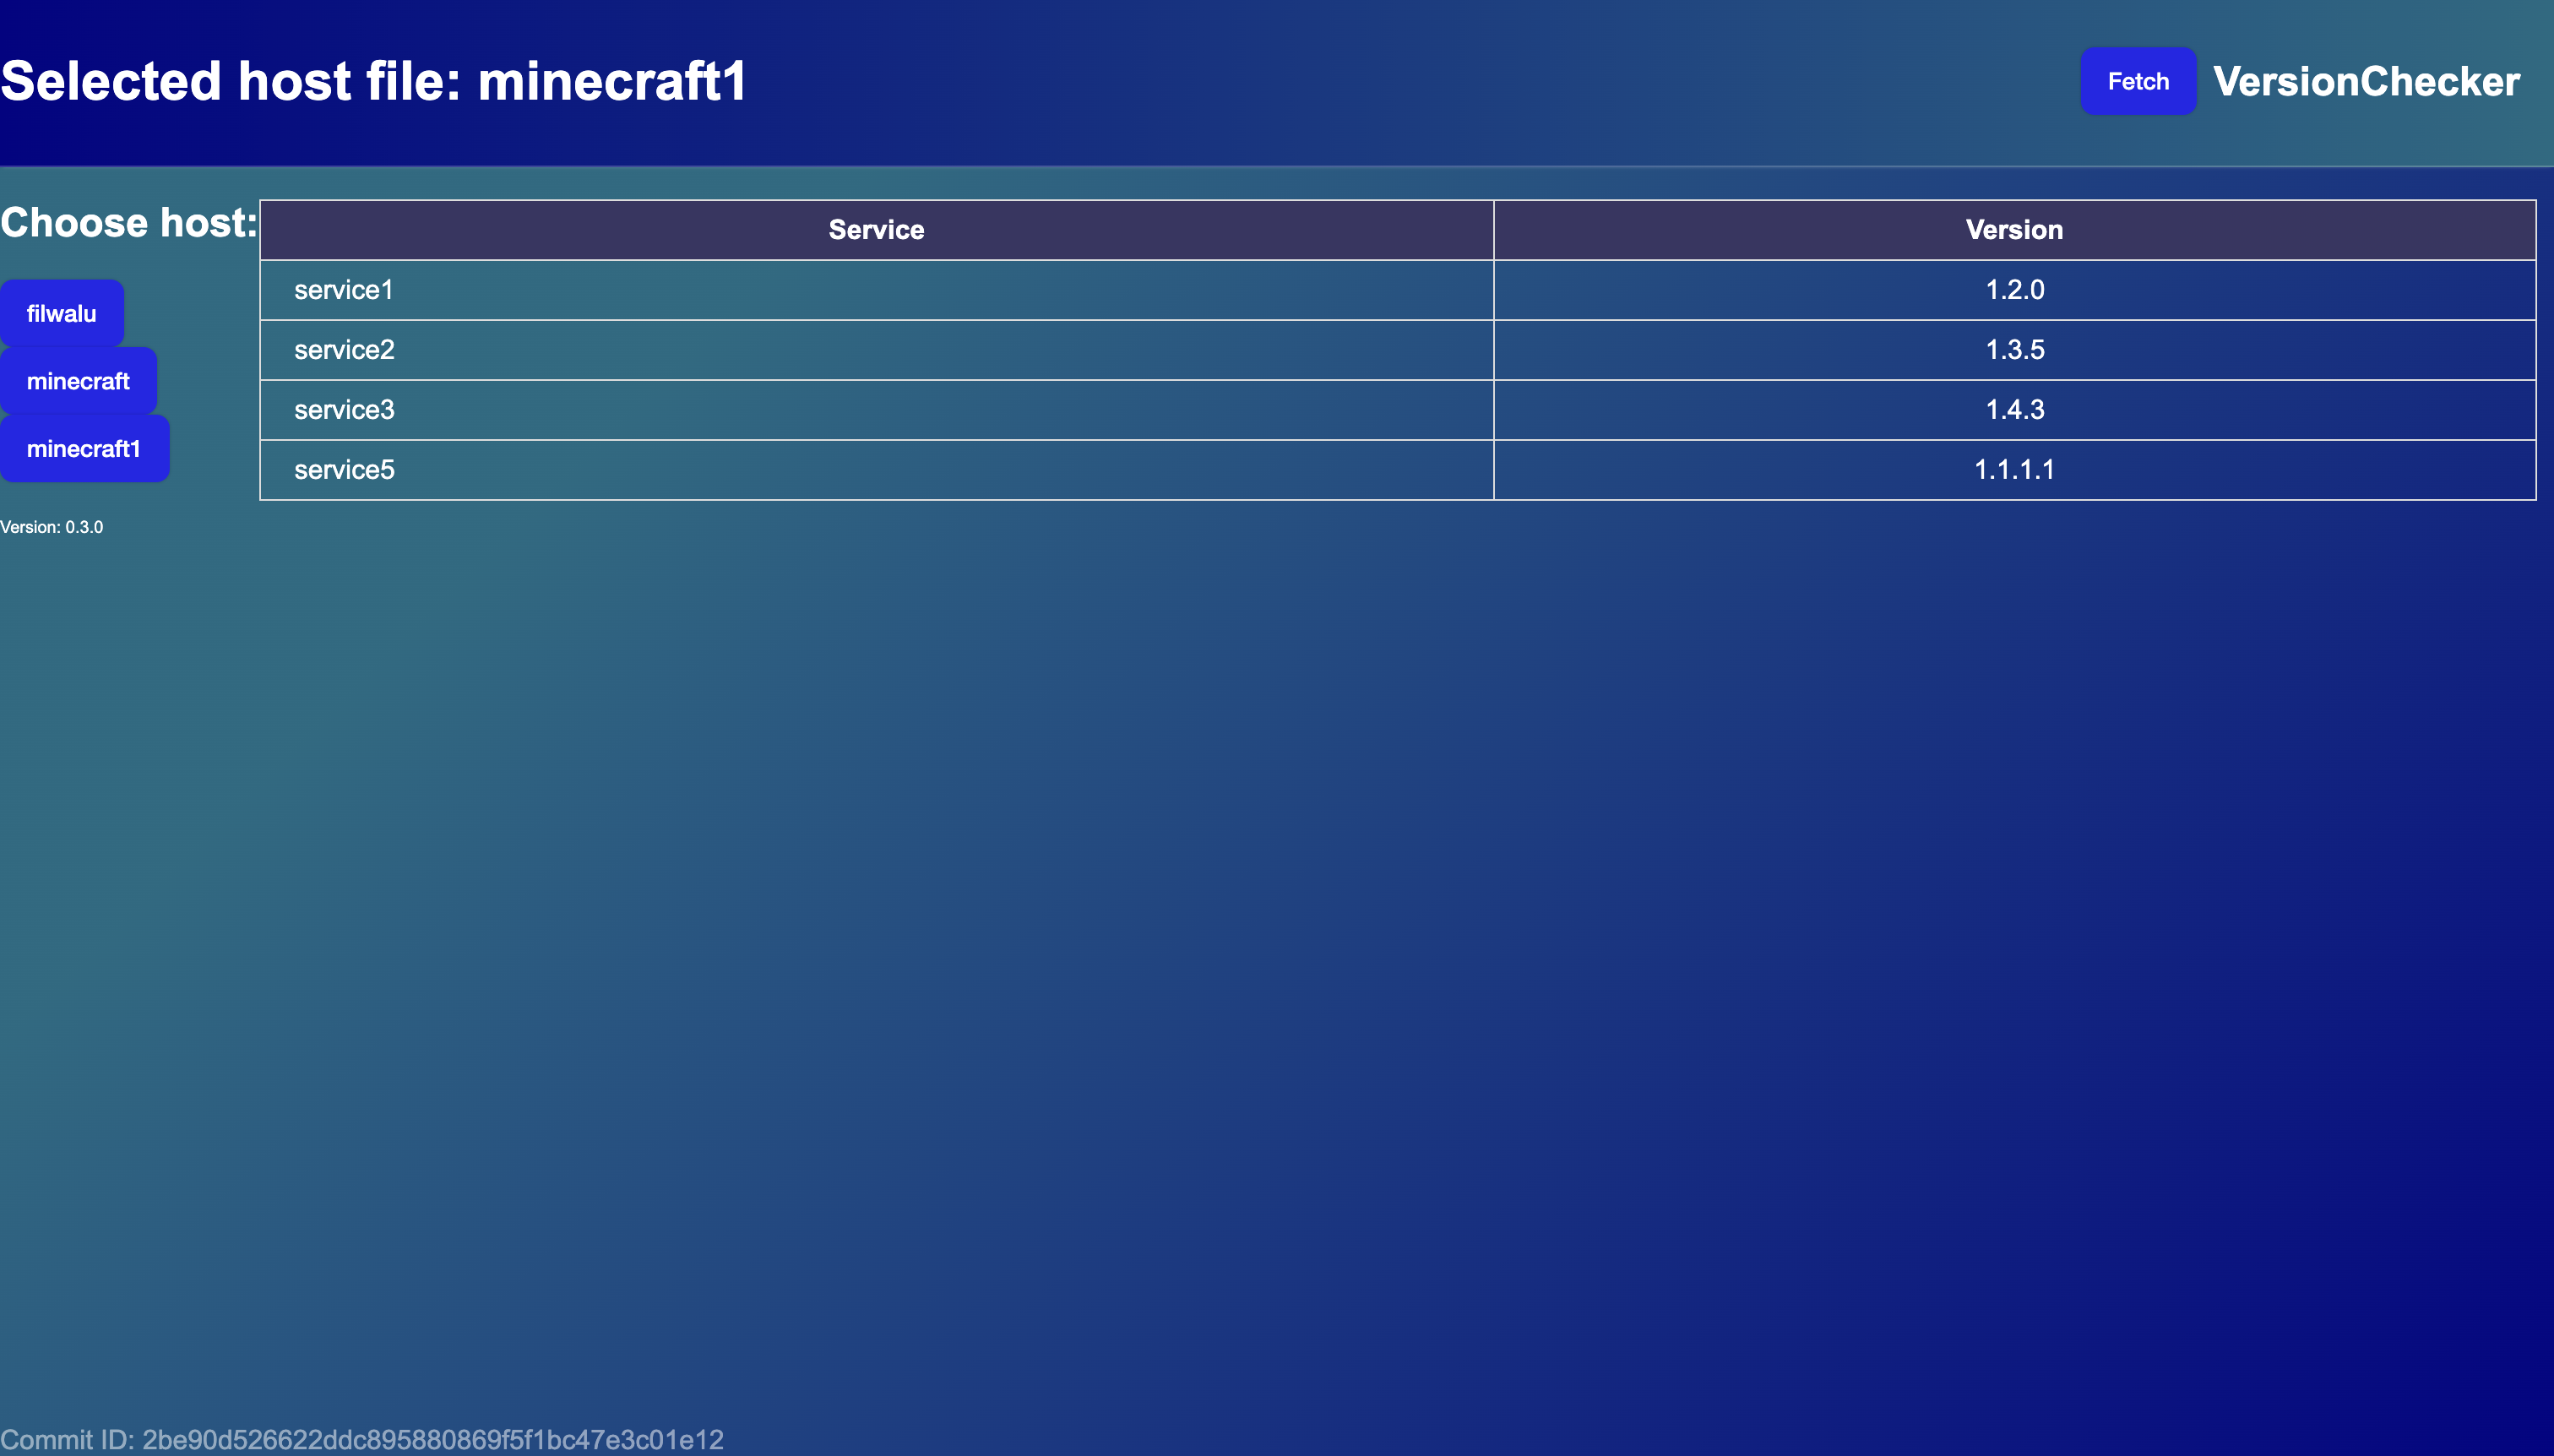
\includegraphics[width=\textwidth]{photos/mainpage.png}
\caption{Strona główna.}
\end{figure}

W tej sekcji omówione zostaną kluczowe funkcjonalności aplikacji instrukcje dotyczące ich używania.

\begin{itemize}
    \item \textbf{Wybór hosta} (\textit{Przyciski z nazwami hostów}):
    Użytkownik może wybrać hosta, którego wersje serwisów chce sprawdzić, klikając na przycisk z nazwą hosta. Po kliknięciu na przycisk, aplikacja wyświetli tabele z nazwami serwisów oraz ich wersjami.
    \begin{figure}[H]
    \centering
    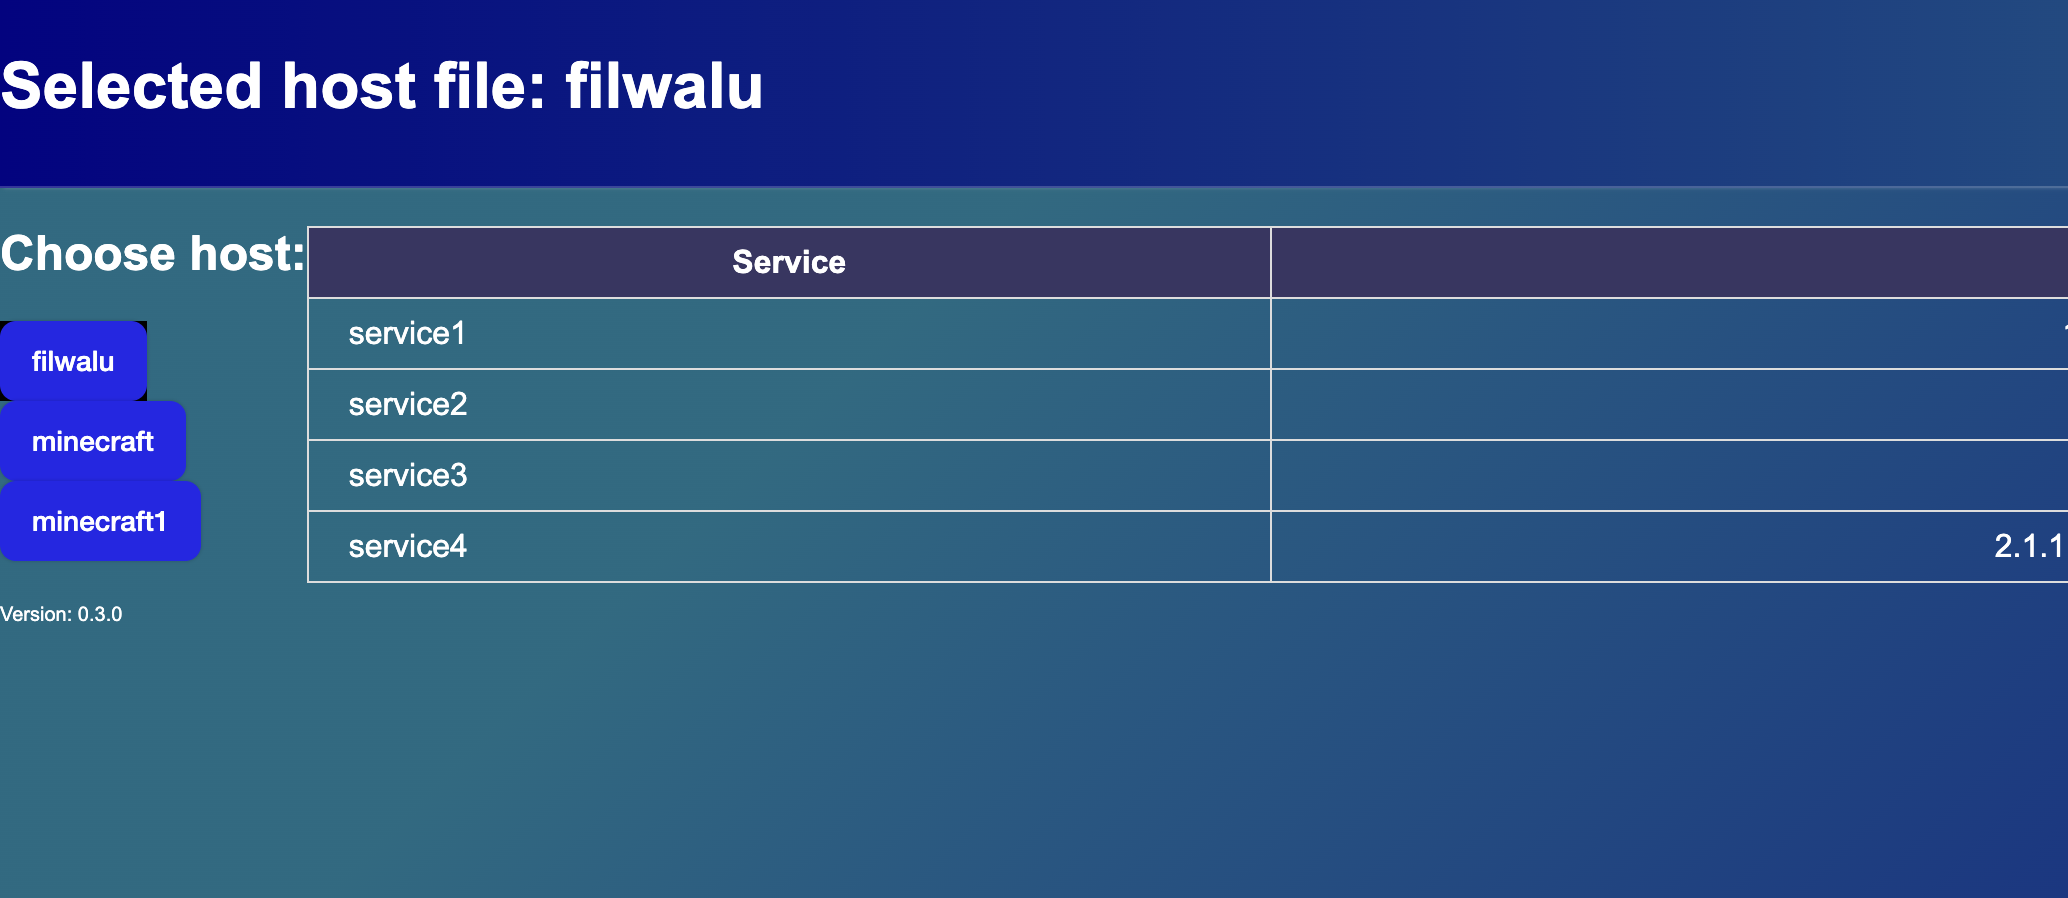
\includegraphics[width=\textwidth]{photos/diffHost.png}
    \caption{Wybór hosta.}
    \end{figure}

    \item \textbf{Pobieranie wersji serwisów} (\textit{Przycisk "Fetch"}):
    Użytkownik może pobrać wersje serwisów dla wybranego hosta, klikając na przycisk "Fetch". Po kliknięciu na przycisk, aplikacja sprawdzi czy wersje serwisów zmieniły się na danym hoście i w razie potrzeby je zaaktualizuje na stronie. 
        \begin{figure}[H]
        \centering
        
\includegraphics[width=\textwidth]{photos/fetchButton.png}
        \caption{Przycisk Fetch.}
        \end{figure}
    \clearpage
    \item \textbf{Status pobierania informacji o wersjach serwisów} (\textit{Komunikat "Update Successful"}):
    Po pobraniu wersji serwisów dla wybranego hosta, aplikacja wyświetli komunikat "Update Successful" informujący użytkownika o pomyślnym pobraniu wersji serwisów.
        \begin{figure}[H]
        \centering
        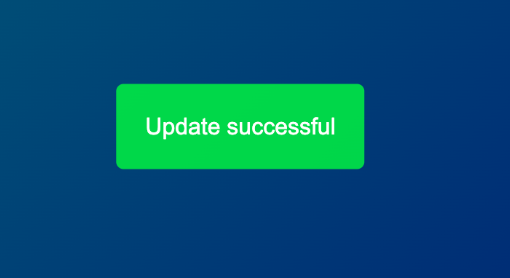
\includegraphics[width=\textwidth]{photos/SUCCESS.png}
        \caption{Komunikat Update Successful.}
        \end{figure}

\end{itemize}
\section{Opis interakcji z użytkownikiem}
Aplikacja skupia się na minimalizmie i łatwości nawigacji, co pozwala na szybkie odnalezienie potrzebnych informacji i funkcji. Interfejs użytkownika jest intuicyjny i prosty w obsłudze, dlatego większość błędów jest logowana do pliku app.log. 

\newpage
\chapter{Podsumowanie}
W ramach projektu Aplikacja pozwalająca na szybkie sprawdzenie wersji serwisów na serwerach Linux szereg prac, w tym:
\begin{itemize}
    \item Implementacja systemu logowania błędów do pliku app.log za pomocą biblioteki loguru.
    \item Uruchomienie prostego serwera www działającego na lokalnym hoście, dzięki bibliotece Flask.
    \item Przygotowanie interfejsu użytkownika na stronie www za pomocą templateów Jinja, kodu CSS oraz JavaScript.
    \item Wykorzystanie plików JSON do przechowywania danych o serwisach i wersjach, oraz docelowych hostach.
    \item Wykorzystanie biblioteki paramiko do obsługi połączeń SSH do docelowych hostów, za pomocą prywatnego klucza.
\end{itemize}


W dalszej kolejności planowane są następujące prace rozwojowe:
\begin{itemize}
    \item Konteneryzacja aplikacji z wykorzystaniem Docker, co ułatwi wdrożenie i skalowalność.
    \item Rozbudowa obsługi wyjątków dla zwiększenia stabilności i niezawodności aplikacji.
    \item Wdrożenie obsługi requestów /POST w celu możliwości dodania pliku hosta bez potrzeby umieszczania go bezpośrednio w plikach.
\end{itemize}

\newpage

% *************** Bibliografia ***************
\begin{thebibliography}{9}

    \bibitem{flaskdocs} 
    Flask Documentation. 
    \textit{Pallets Projects}. 
    Available at: \url{https://flask.palletsprojects.com/en/3.0.x/}.
    
    \bibitem{paramikodocs} 
    Paramiko Documentation. 
    \textit{Paramiko Development Team}. 
    Available at: \url{https://docs.paramiko.org/en/latest/}.
    
    \bibitem{jinja2docs} 
    Jinja Documentation. 
    \textit{Pallets Projects}. 
    Available at: \url{https://jinja.palletsprojects.com/en/3.1.x/}.
\end{thebibliography}
\newpage

% *************** Zakończenie ***************
\addcontentsline{toc}{chapter}{Spis rysunków}
\listoffigures
\newpage


\end{document}
% *************** Koniec pliku szablon.tex ***************
